\documentclass[unknownkeysallowed,usepdftitle=false]{beamer}
% unknownkeysallowed is needed for mac and the newer latex version -> is more picky than before...
\usetheme[headheight=1cm,footheight=2cm]{boxes}
%\usetheme{default}

\usepackage{inputenc}
\usepackage{default}
\usepackage{graphicx}
\usepackage{epsfig}
\usepackage{siunitx}
\usepackage{color}
\usepackage{ifthen}
\usepackage{ragged2e}
\usepackage{animate}

\setbeamertemplate{navigation symbols}{}%remove navigation symbols
\setbeamersize{text margin left=0pt,text margin right=0pt} % text and figures flush to edges

% some colors
\definecolor{grau}{gray}{.5}
\definecolor{slfcolor}{rgb}{0,0.5,0.8353}
\definecolor{wslcolor}{rgb}{0,0.4,0.4}

% setup links
\hypersetup{%
	%linkbordercolor=green,%
	colorlinks=false,%
	pdfborderstyle={/S/U/W 0},%
	%pdfpagemode=FullScreen,%
	pdfstartpage=4%
	}

% setup some fonts
\setbeamerfont{title}{series=\bfseries, size=\small}
\setbeamerfont{author}{size*={5pt}{0pt}}
\setbeamerfont{institute}{size*={3pt}{0pt}}
\setbeamerfont{bodytext}{size=\scriptsize}


% Title setup	
\title{Absolute Velocity Estimates from a Glider Mounted ADCP}
\author{Callum Rollo\inst{1} (\texttt{c.rollo@uea.ac.uk}) \and Karen J Heywood\inst{1} \and Rob Hall\inst{1} \and Alex Phillips\inst{2}}
\institute{\inst{1}University of East Anglia, Norwich, UK
\quad \inst{2}Marine Autonomous Robotics Systems group, Southampton UK}
% add title in headbox
\setbeamertemplate{headline}
{\leavevmode
\begin{beamercolorbox}[width=1\paperwidth]{head title}
  % LOGOS
  \begin{columns}[t, totalwidth=\textwidth]
  \begin{column}[c]{0.35cm}
     
\includegraphics[height=1.05cm]{figure/graphic_egu_photo_yes.png}
  \end{column}
  \begin{column}[c]{0.8cm}
     
\includegraphics[height=1.05cm]{figure/egu_ospp_label_blue.png}
  \end{column}

  % TITLE
   \begin{column}[c]{9.6cm}
   \centering \usebeamerfont{title} \textcolor{slfcolor}{\inserttitle} \\
   \centering \usebeamerfont{author} \color[rgb]{0,0,0} \insertauthor \\
   \vspace{-0.05cm}
   \centering \usebeamerfont{institute} \insertinstitute
  \end{column}
  % PICUTRE
  \begin{column}[c]{0.9cm}
    \hspace{0.005cm}
    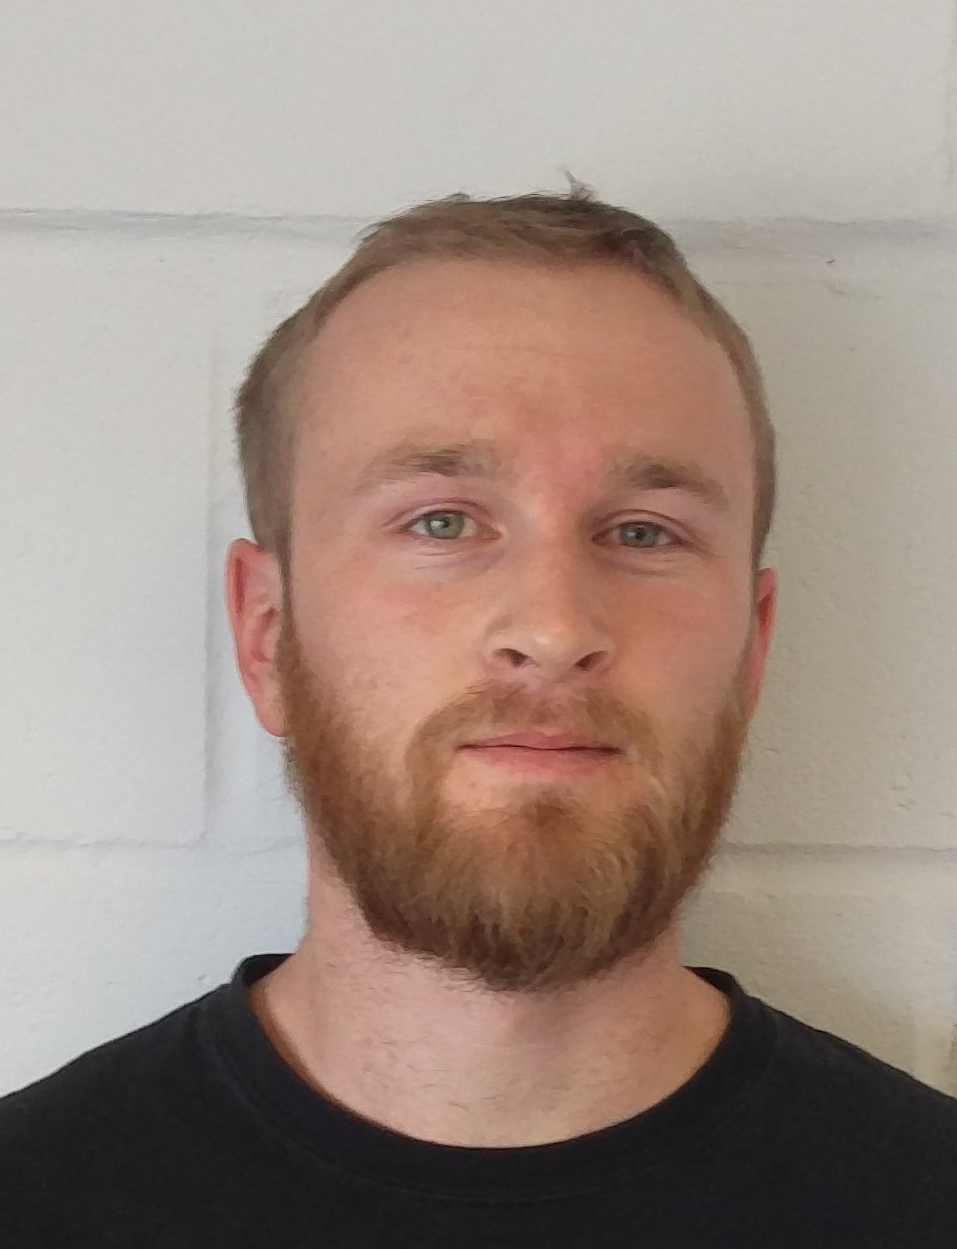
\includegraphics[trim=0 0 0 0,clip,height=1.05cm]{figure/mug.jpg}
  \end{column}
  \end{columns}
  {\color{slfcolor}\hrule height 1pt\vspace{0.1cm}}
\end{beamercolorbox}%
}

% setup the navigation in footbox
% first set some button colors
\newcommand{\buttonactive}{\setbeamercolor{button}{bg=wslcolor,fg=white}}
\newcommand{\buttonpassive}{\setbeamercolor{button}{bg=slfcolor,fg=white}}
% now set up that the one active one gets the new color.
\newcommand{\secvariable}{nothing}
% therefore we write before each section (well, everything which should be part of the navi bar)
% the variable \secvariable to any name which is in the next function ...
\newcommand{\mysection}[1]{\renewcommand{\secvariable}{#1}
}
% ... compaired to strings in the following navibar definition ...
\newcommand{\tocbuttoncolor}[1]{%
 \ifthenelse{\equal{\secvariable}{#1}}{%
    \buttonactive}{%
    \buttonpassive}
 }
% ... here we start to set up the navibar. each entry is calling first the function \tocbuttoncolor with the argument which should be tested for being active. if active, then change color. afterwards the button is draw. so to change that, you need to change the argument in \toc..color, the first in \hyperlink and before each frames definition... A bit messed up, but works...
\newlength{\buttonspacingfootline}
\setlength{\buttonspacingfootline}{-0.2cm}
\setbeamertemplate{footline}
{\leavevmode
\begin{beamercolorbox}[width=1\paperwidth]{head title}
  {\color{slfcolor}\hrule height 1pt}
  \vspace{0.05cm}
  % set up the buttons in an mbox
  \centering \mbox{
    \tocbuttoncolor{intro}
    \hyperlink{intro}{\beamerbutton{Introduction}}
    \tocbuttoncolor{trial_shear}
    \hspace{\buttonspacingfootline}
      \hyperlink{trial_shear}{\beamerbutton{Trials results}}
    \tocbuttoncolor{rationale}
    \hspace{\buttonspacingfootline}
      \hyperlink{rationale}{\beamerbutton{Rationale \& aims}}
    \tocbuttoncolor{plan}
    \hspace{\buttonspacingfootline}
      \hyperlink{plan}{\beamerbutton{Deployment plan}}
    \tocbuttoncolor{qc}
    \hspace{\buttonspacingfootline}
      \hyperlink{qc}{\beamerbutton{Data qc}}
    \tocbuttoncolor{tech}
    \hspace{\buttonspacingfootline}
      \hyperlink{tech}{\beamerbutton{Tech specs}}

    % this last one should normaly not be used... it will open the preferences to change the 
    % behaviour of the acrobat reader in fullscreen -> usefull in pico...
    \setbeamercolor{button}{bg=white,fg=black}
    % for presentation
    %\hspace{-0.1cm}\Acrobatmenu{FullScreenPrefs}{\beamerbutton{\#}}
    % for upload
    
     
\Acrobatmenu{FullScreenPrefs}{\vspace{0.3cm}\hspace{0.24cm}\mbox{%
      \includegraphics[height=0.04\textheight,keepaspectratio]{%
	  figure/CreativeCommons_Attribution_License}%
	  }}
   }
    \vspace{0.05cm}
\end{beamercolorbox}%
}



\begin{document}


%%%%%%%%%%%%%%%%%%%%%%%%%%%%%%%%%%%%%%%%%%%%%%%%%%%%%%%%%%%%%%%%%%%%%%%%%%
\mysection{intro}
%%%%%%%%%%%%%%%%%%%%%%%%%%%%%%%%%%%%%%%%%%%%%%%%%%%%%%%%%%%%%%%%%%%%%%%%%%
\begin{frame}\label{\secvariable}
\usebeamerfont{bodytext}
\justifying

\vspace*{-1.2mm}    

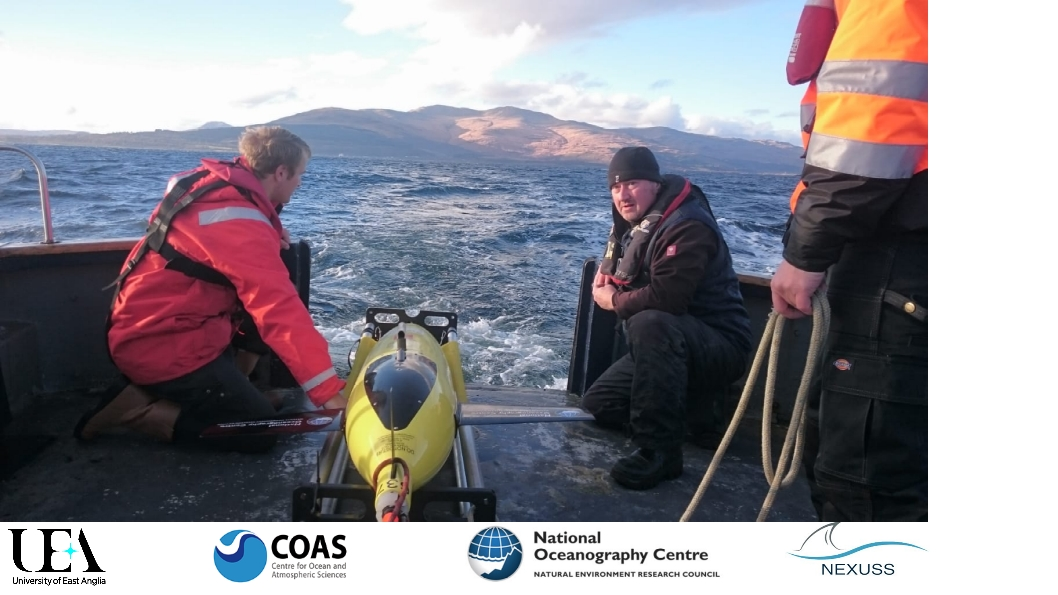
\includegraphics[trim=0 0 100 5,clip,width=\paperwidth]{figure/splash.jpg}


\end{frame}


\begin{frame}\label{animation}

\animategraphics[trim=200 103 170 80,clip,autoplay,width=\paperwidth]{5}{./ani_png/bar}{1}{101}

\end{frame}


%%%%%%%%%%%%%%%%%%%%%%%%%%%%%%%%%%%%%%%%%%%%%%%%%%%%%%%%%%%%%%%%%%%%%%%%%%
\mysection{trial_shear}
%%%%%%%%%%%%%%%%%%%%%%%%%%%%%%%%%%%%%%%%%%%%%%%%%%%%%%%%%%%%%%%%%%%%%%%%%%
\begin{frame}\label{\secvariable}
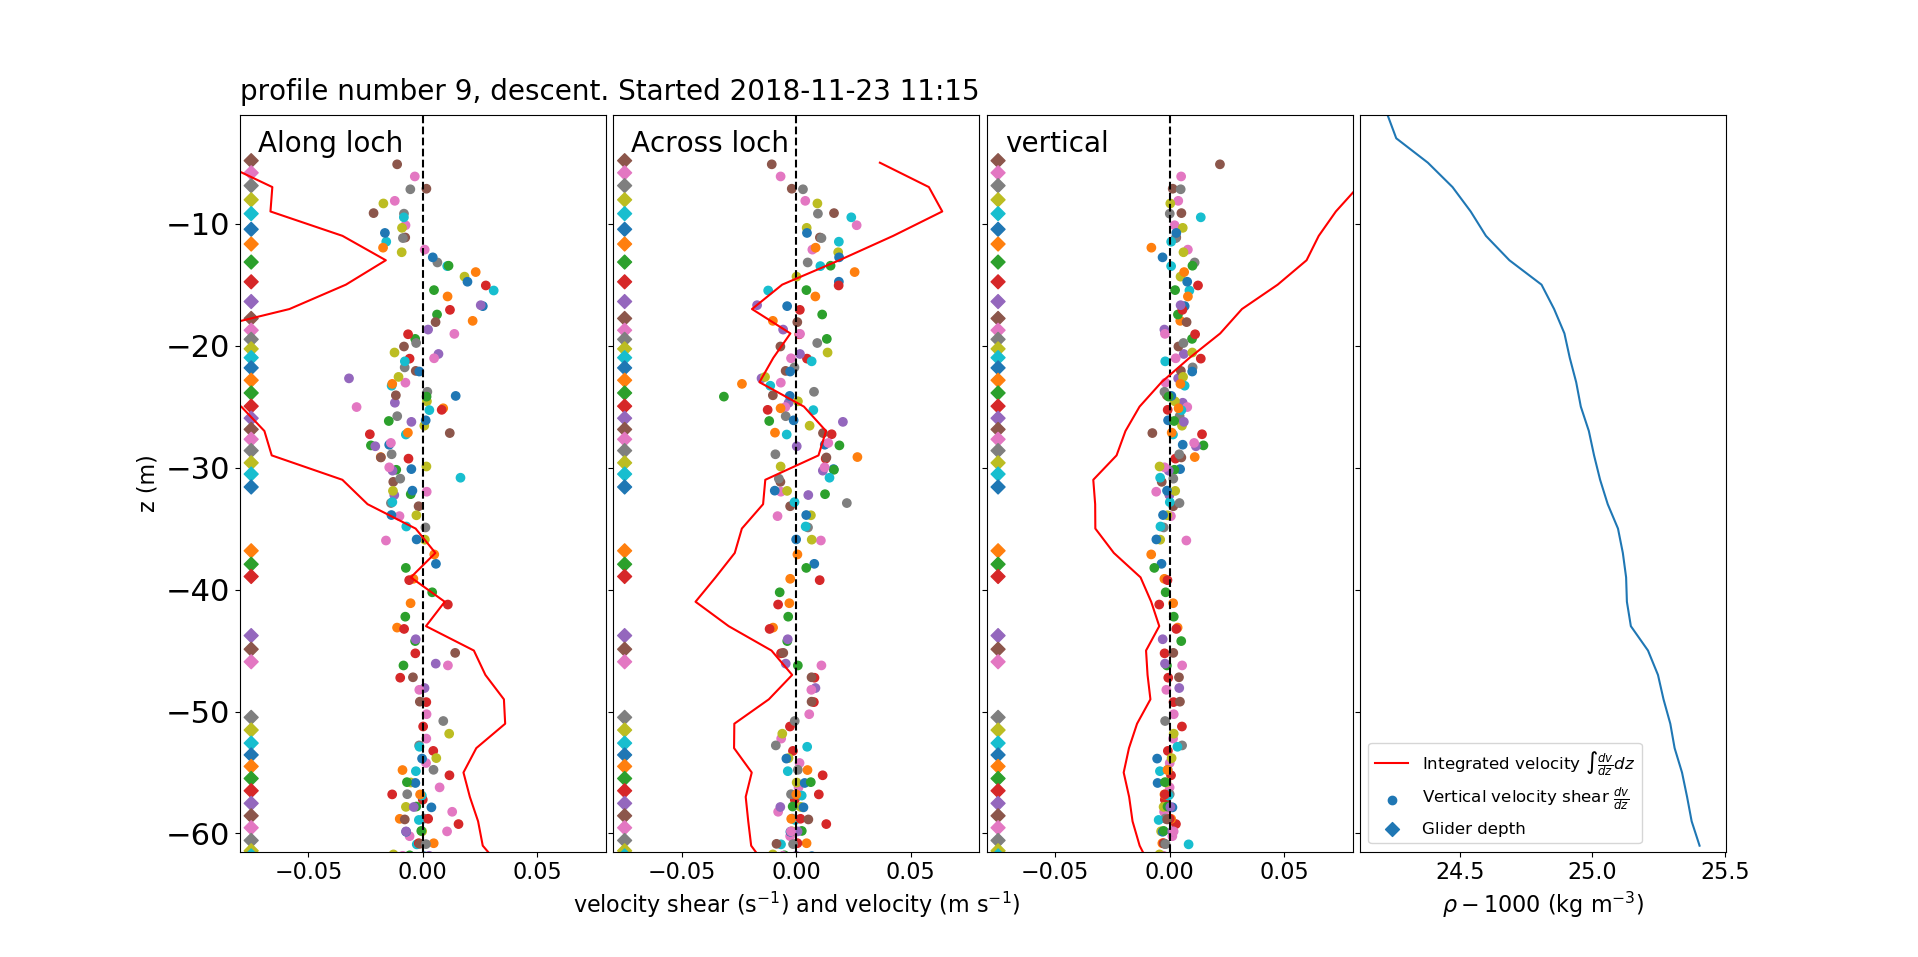
\includegraphics[trim=70 20 80 80,clip,width=\paperwidth]{figure/95_qc.png}
\vspace*{-5mm}
\begin{columns}
\begin{column}[t]{0.9\textwidth}

\scriptsize Velocity shear coloured by the depth of the glider during at the time of the ensemble
\end{column}
\end{columns}



\begin{itemize}
\item Vertical shear of horizontal velocity coherent between ensembles
\item Strong along loch shear across pycnocline
\end{itemize}
  
\end{frame}


\begin{frame}\label{sawtooth}
\vspace*{-1.2mm}    
\begin{center}
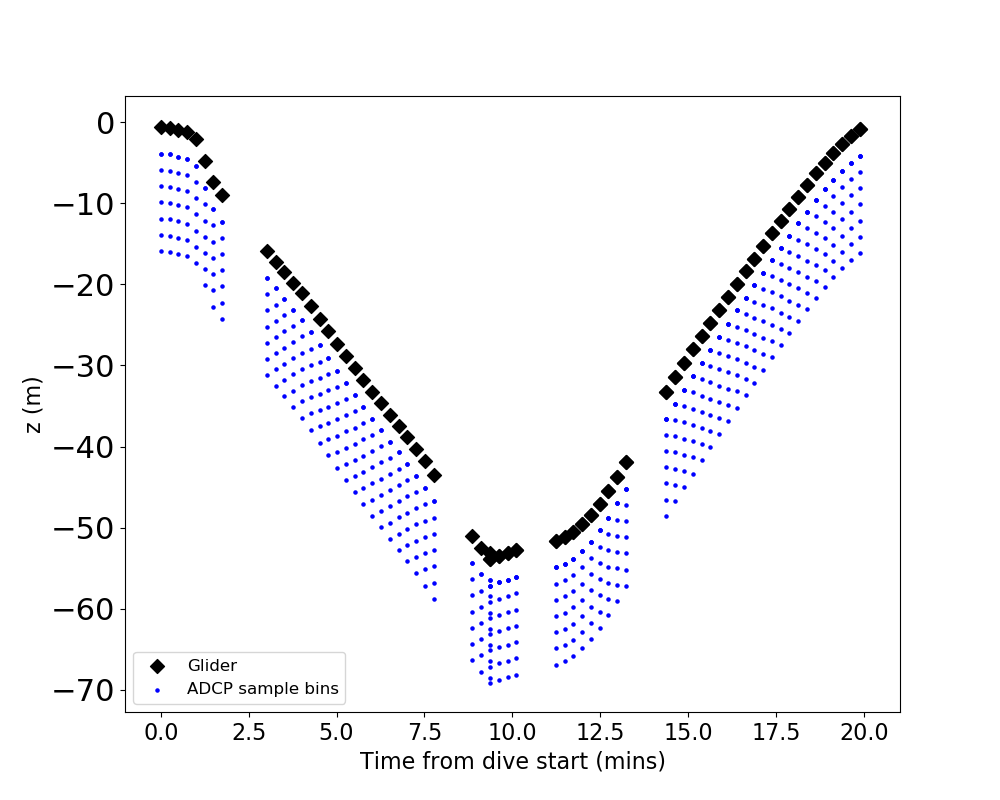
\includegraphics[trim=0 0 0 50,clip,width=0.8\paperwidth]{figure/sawtooth.png}
\end{center}

\vspace*{-5.2mm}
\begin{columns}
\begin{column}[t]{0.9\textwidth}
Dive profile from trials with glider depth and bins out to 15 m plotted
\end{column}
\end{columns}


  
\end{frame}

\begin{frame}\label{3_dives}
\vspace*{-1.2mm}    
\begin{center}
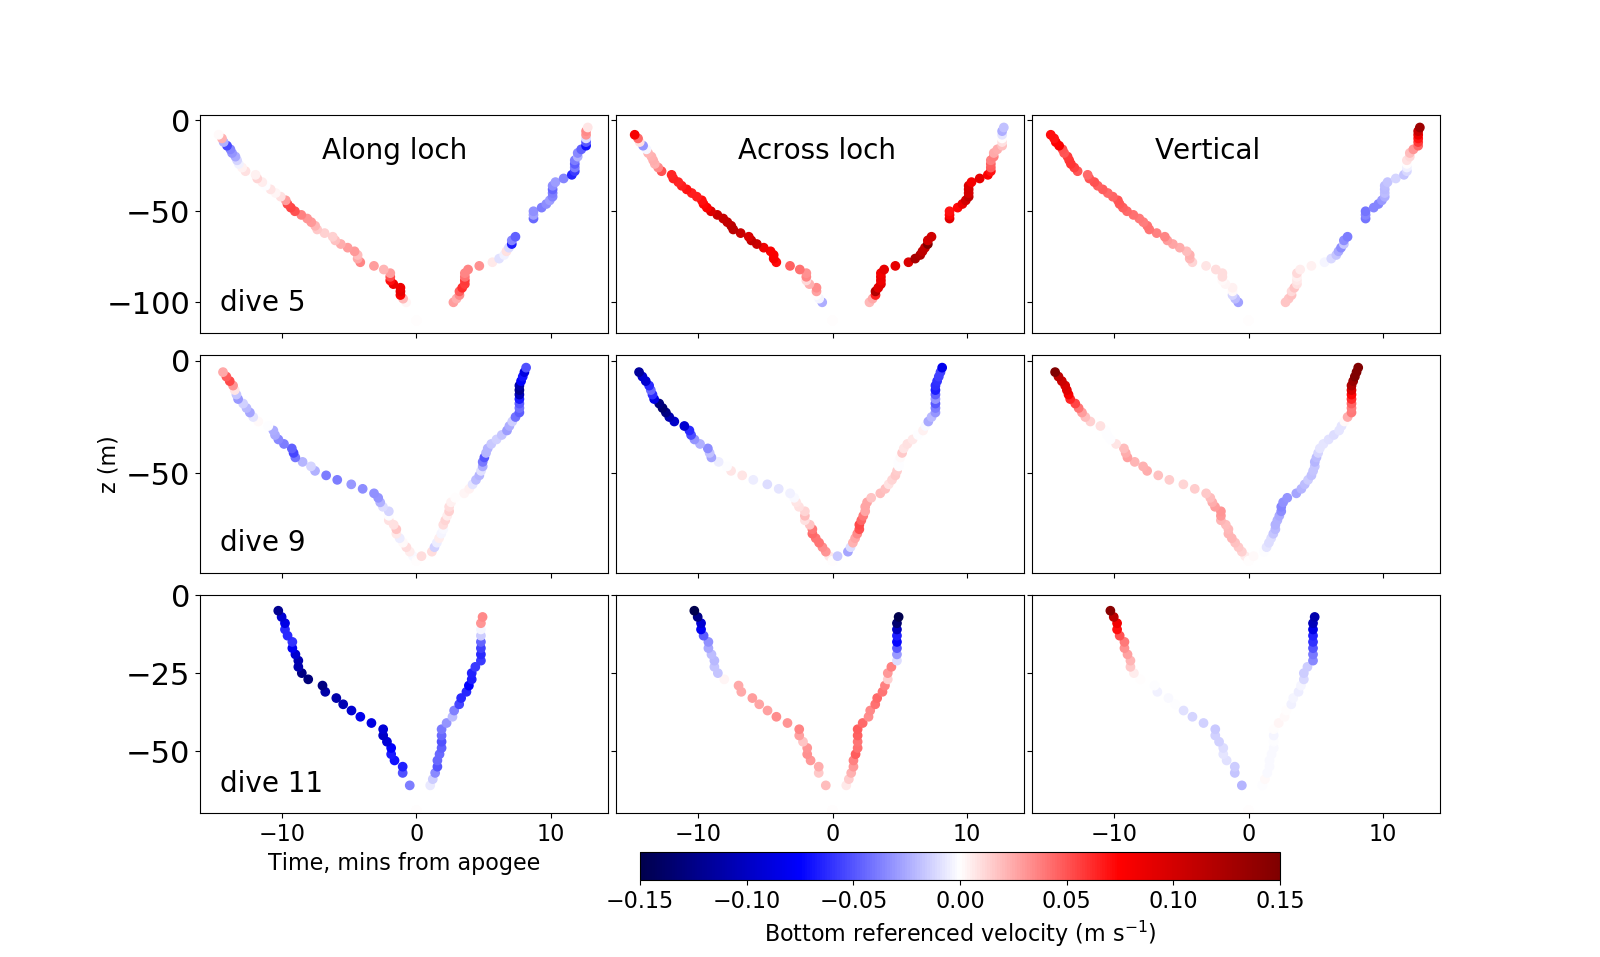
\includegraphics[trim=0 0 0 50,clip,width=\paperwidth]{figure/diveclimb_vel9.png}
\end{center}

\vspace*{-5.2mm}
\begin{columns}
\begin{column}[t]{0.9\textwidth}
Good agreement for horizontal velocities between descents and ascents
\end{column}
\end{columns}



  
\end{frame}

%%%%%%%%%%%%%%%%%%%%%%%%%%%%%%%%%%%%%%%%%%%%%%%%%%%%%%%%%%%%%%%%%%%%%%%%%%
\mysection{rationale}
%%%%%%%%%%%%%%%%%%%%%%%%%%%%%%%%%%%%%%%%%%%%%%%%%%%%%%%%%%%%%%%%%%%%%%%%%%
\begin{frame}\label{\secvariable}

\vspace*{-5.2mm}
\begin{columns}
\begin{column}[t]{0.9\textwidth}

Presently, current velocities are directly measured primarily using moored ADCPs. These systems are reliable but come with drawbacks that we hope to address by using a glider instead:

\begin{itemize}
\item Moorings are often "trawled out" by fishing activity, a glider is much less vulnerable.
\item Recovering and replacing moorings requires expensive ship time. Gliders can be launched and recovered from cheap, small vessels.
\item Upward facing moored ADCPs suffer from reflections near the surface, the downward facing ADCP on a glider does not.
\item As they profile, gliders collect  salinity and temperature data every 5 s. Analysing this with coincident shear is of great scientific value.
\item The higher frequency glider ADCP (1MHz vs 55 kHz) can resolve smaller features in current shear. \hyperlink{tech}{\beamerbutton{see tech specs}}
\end{itemize}
\end{column}
\end{columns}



  
\end{frame}
%%%%%%%%%%%%%%%%%%%%%%%%%%%%%%%%%%%%%%%%%%%%%%%%%%%%%%%%%%%%%%%%%%%%%%%%%%
\mysection{plan}
%%%%%%%%%%%%%%%%%%%%%%%%%%%%%%%%%%%%%%%%%%%%%%%%%%%%%%%%%%%%%%%%%%%%%%%%%%
\begin{frame}\label{\secvariable} %%Eine Folie
\vspace{-0.3cm}
\begin{center}
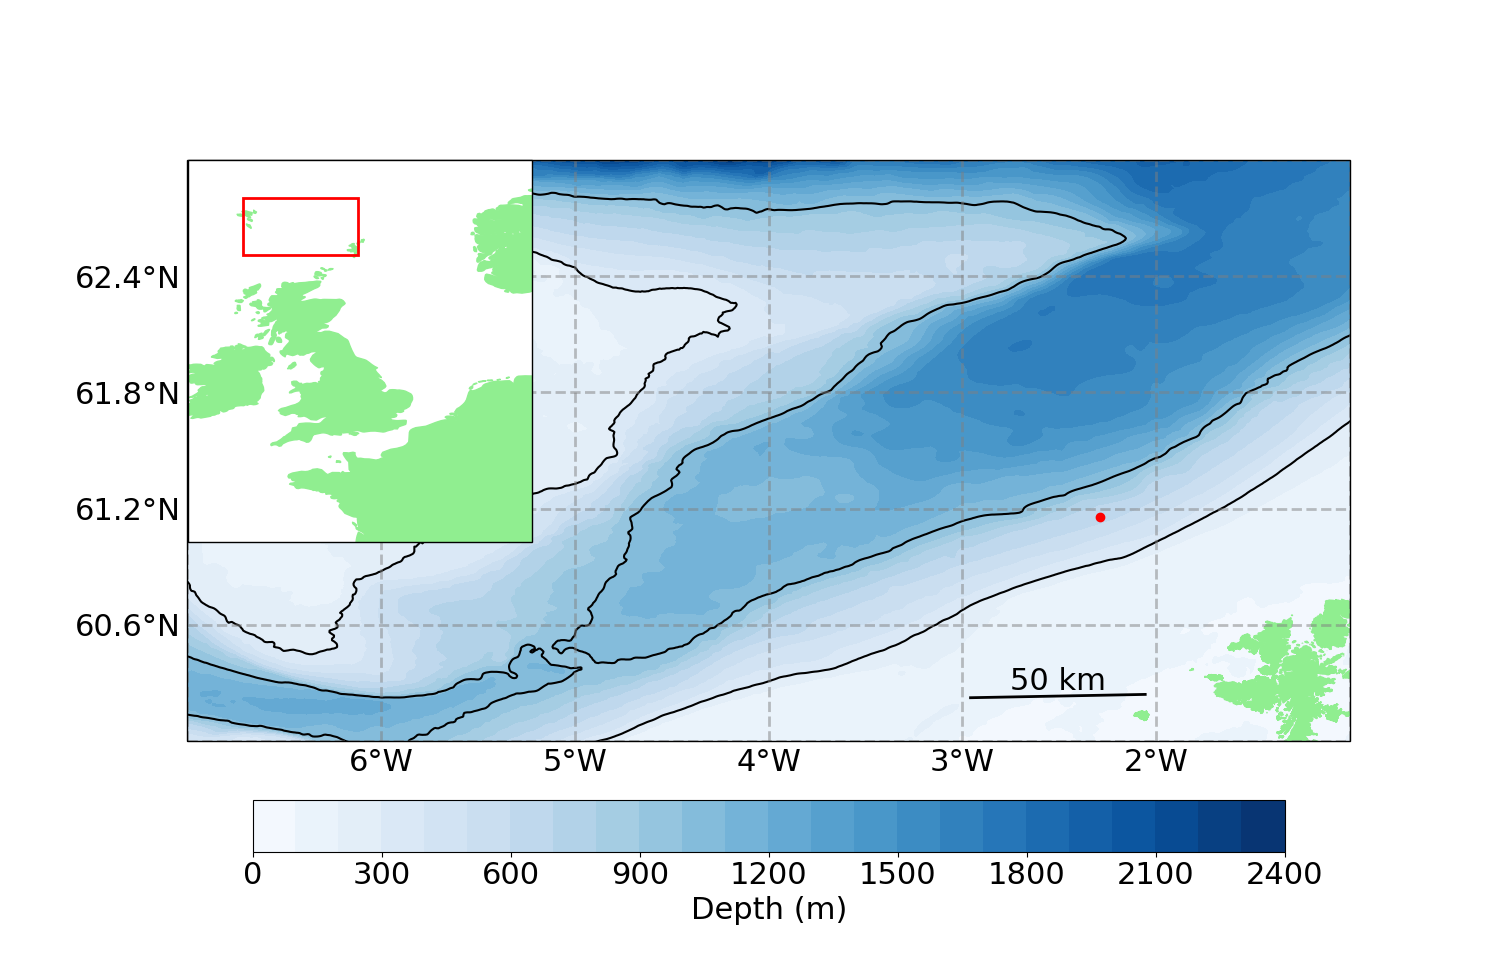
\includegraphics[trim=0 10 0 110,clip,width=1\textwidth,keepaspectratio]{%
figure/basemap.png}
\end{center}
\begin{columns}
\begin{column}[t]{0.9\textwidth}
Red dot marks planned deployment to the Faroe Shetland Channel April 2019 \hyperlink{dep_details}{\beamerbutton{more details}} \hyperlink{fsc_shear}{\beamerbutton{see expected conditions}}
\end{column}
\end{columns}
\end{frame}

\begin{frame}\label{dep_details} %%Eine Folie
\vspace{-0.3cm}
\begin{center}

\begin{columns}
\begin{column}[t]{0.9\textwidth}
\begin{itemize}
\item Glider will be deployed for $14+$ days to resolve a tidal cycle at a point on the slope in 600 m depth of water.
\item At the same location we will deploy a 55 kHz moored ADCP to validate the shear velocities estimated from the glider.
\item A Pressure Inverted Echo Sounder (PIES) will also be deployed with the moored ADCP, this will provide information of sea surface height, sound velocity and thermocline location at high temporal resolution to complement glider data.
\item We expect to resolve the spring-neap cycle and hope to see evidence of internal tides and solibores.
\item If successful, the glider will transit to another nearby mooring and repeat the procedure, collecting shear velocity profiles between the two moorings 
\end{itemize}
\end{column}
\end{columns}
\end{center}
\end{frame}


\begin{frame}\label{fsc_shear}
\vspace*{-10mm}    
\begin{center}
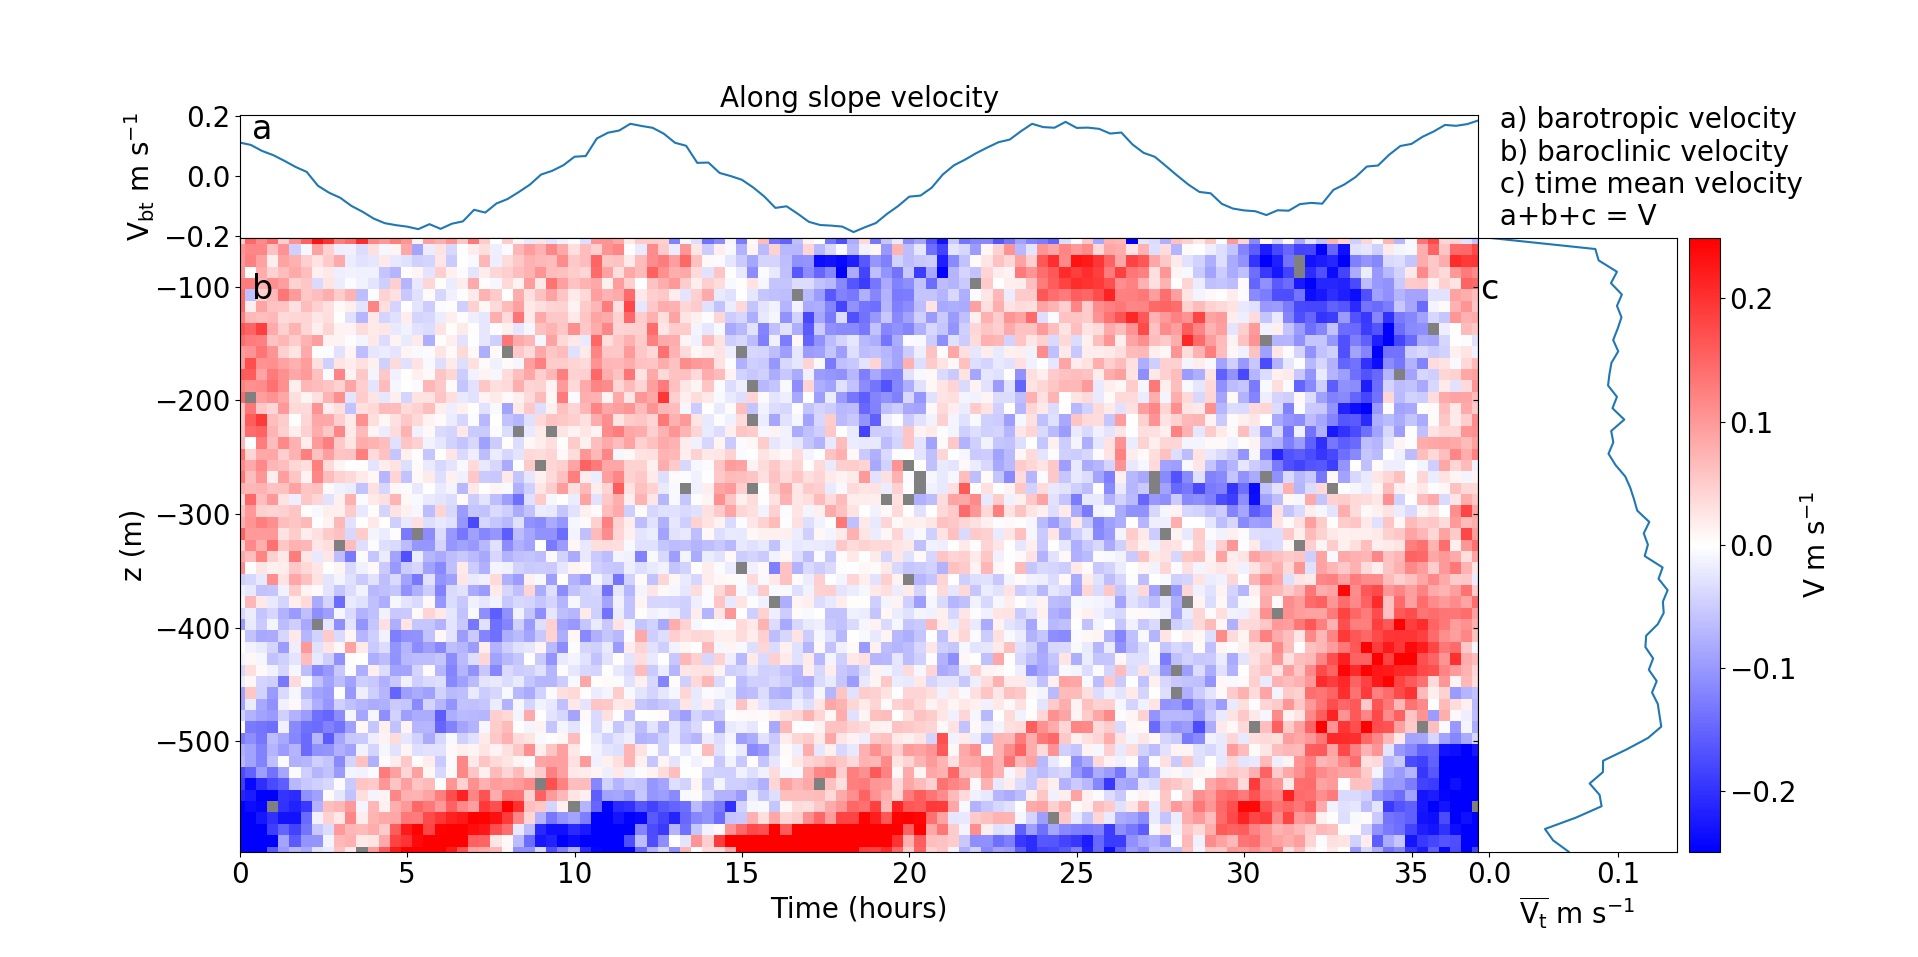
\includegraphics[trim=20 20 20 60,clip,width=\paperwidth]{figure/adcp_fsc.png}
\end{center}
\vspace*{-5mm}    
\begin{columns}
\begin{column}[t]{0.9\textwidth}
55 kHz moored ADCP data from the deployment location. Tidal currents of $0.2\ \mathrm{m\ s^{-1}}$ and bottom intensified baroclinic flows expected.

ADCP data courtesy of Bee Berx, Marine Scotland Science
\end{column}
\end{columns}
 
\end{frame}
%%%%%%%%%%%%%%%%%%%%%%%%%%%%%%%%%%%%%%%%%%%%%%%%%%%%%%%%%%%%%%%%%%%%%%%%%%
\mysection{qc}
%%%%%%%%%%%%%%%%%%%%%%%%%%%%%%%%%%%%%%%%%%%%%%%%%%%%%%%%%%%%%%%%%%%%%%%%%%
\begin{frame}\label{\secvariable}
\ \textbf{Quality control  and calculation steps}
\begin{itemize}
\item Discard cells where glider attitude causes beam miss of $> 1$ m as the beams will be sampling different bins \hyperlink{flight_envelope}{\beamerbutton{see plot}}
\item Discard cells where the ping correlation is less than 50\%
 \hyperlink{ping_corr}{\beamerbutton{see plot}}
\item Rotate from beam coordinates to East-North-Up using data from attitude sensors and compass on the ADCP
\item Calculate shear between adjacent sampling cells in each ensemble
\item Average shear data from all ensembles of the dive in 2 m vertical bins
\item Integrate shear to get relative velocity profiles
\item Reference relative velocity profiles using dive average current from the glider for "absolute" velocity profiles

\end{itemize}
\ What if we don't apply this quality control? \hyperlink{no_qc}{\beamerbutton{see plot}}
\end{frame}


\begin{frame}\label{flight_envelope}
\vspace{-0.3cm}
\begin{center}
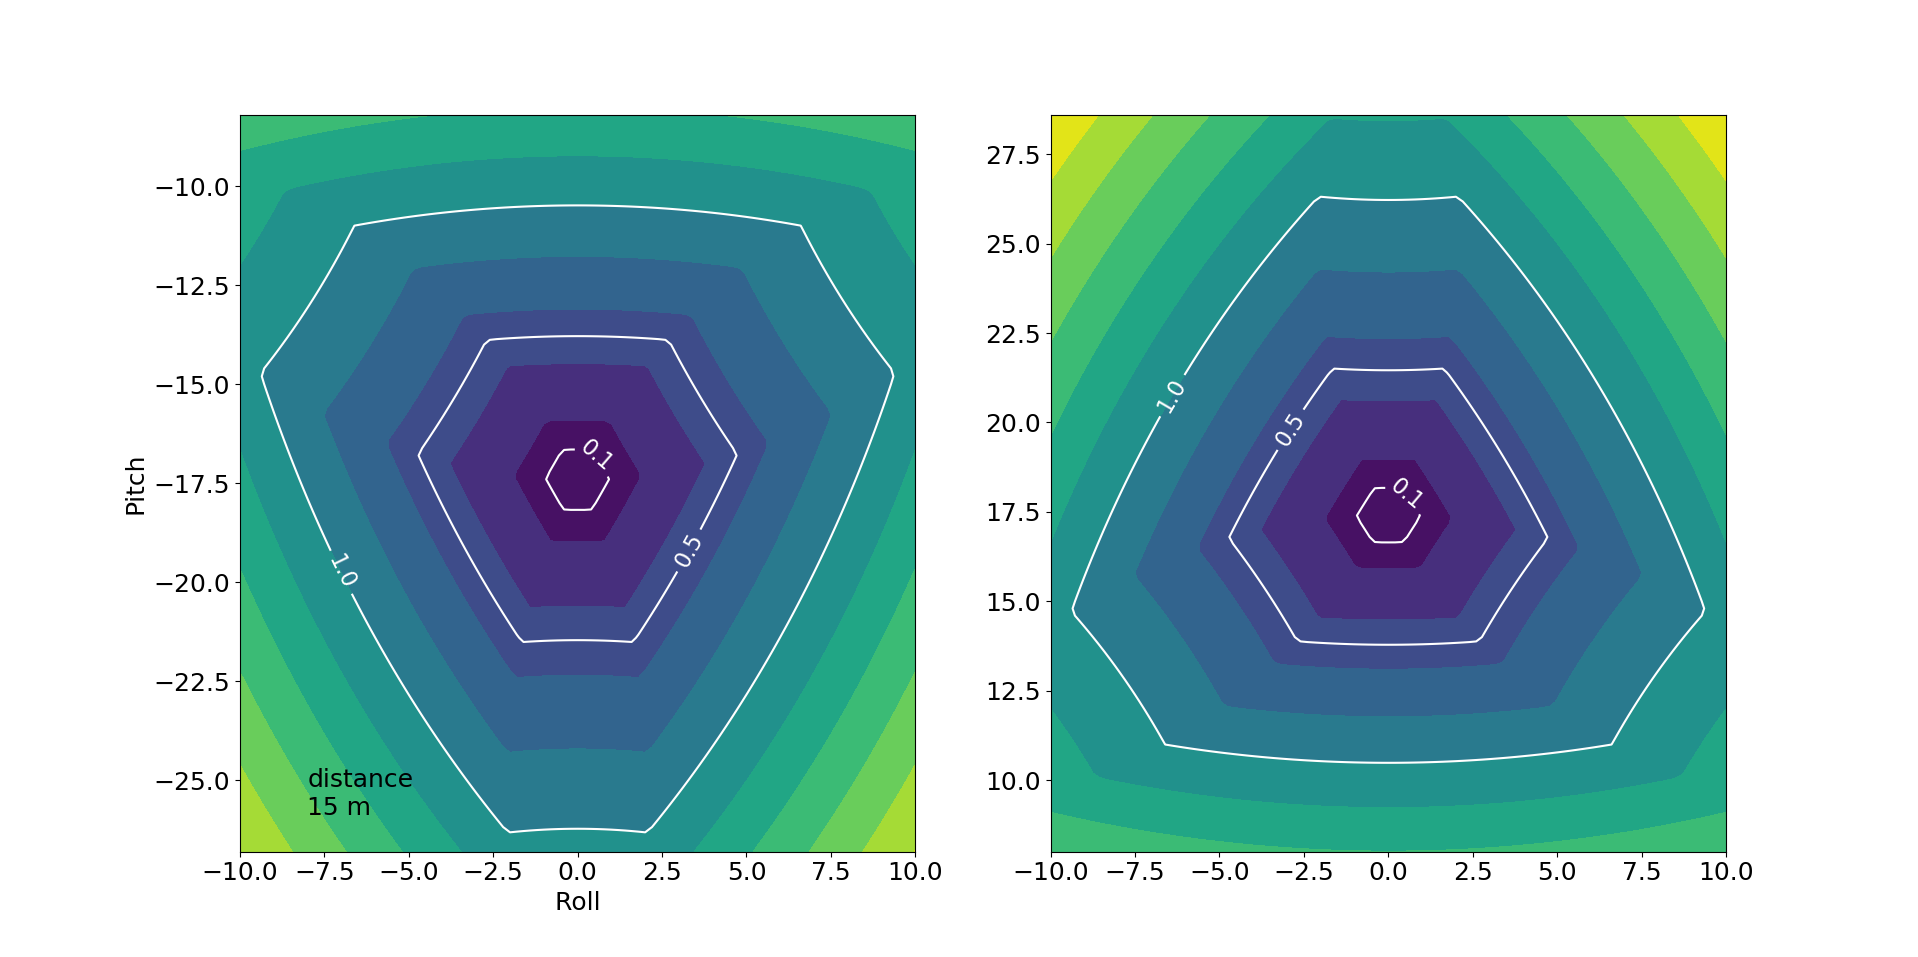
\includegraphics[trim=0 10 0 50,clip,width=1\textwidth,keepaspectratio]{%
figure/flight_aim.png}
\end{center}
\vspace{-0.3cm}
\begin{columns}
\begin{column}[t]{0.9\textwidth}
Flight angle affects the vertical location of the three beams. Plot shows the vertical distance between beams sampling a cell 15 m from the glider over a range of pitch and roll angles. Perfect sampling is achieved at $\pm17.3^{\circ}$ pitch $0^{\circ}$ roll \hyperlink{dive_flight}{\beamerbutton{show me an example}}
\end{column}
\end{columns}
\end{frame}

\begin{frame}\label{dive_flight}
\vspace{-0.3cm}
\begin{center}
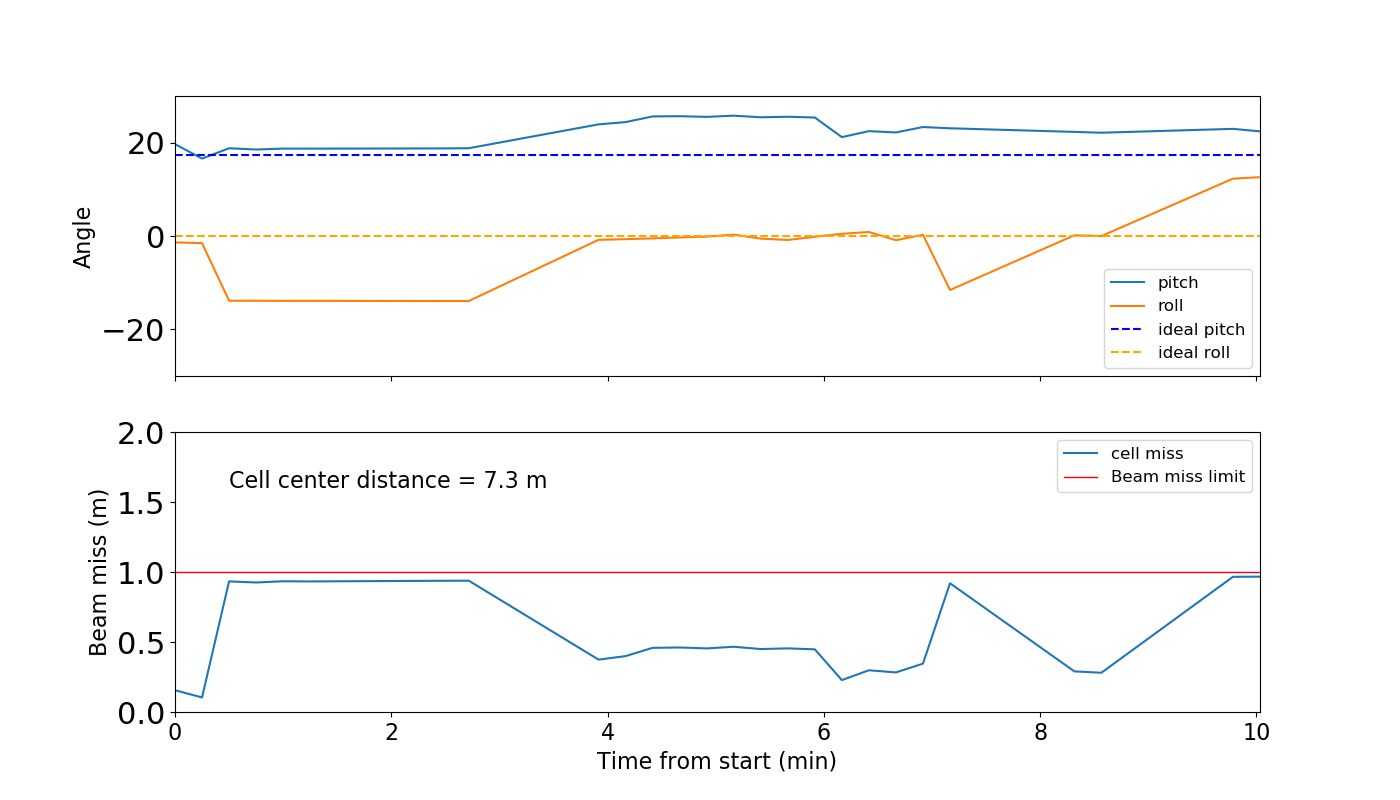
\includegraphics[trim=0 10 0 50,clip,width=1\textwidth,keepaspectratio]{%
figure/flight_miss.png}
\end{center}
\vspace{-0.3cm}
\begin{columns}
\begin{column}[t]{0.9\textwidth}
Example ascent profile shows the difficulty of keeping the glider within the acceptable pitch and roll envelope \hyperlink{flight_envelope}{\beamerbutton{see plot}}, especially on short dives 
\end{column}
\end{columns}
\end{frame}


\begin{frame}\label{ping_corr}
\vspace{-0.3cm}
\begin{center}
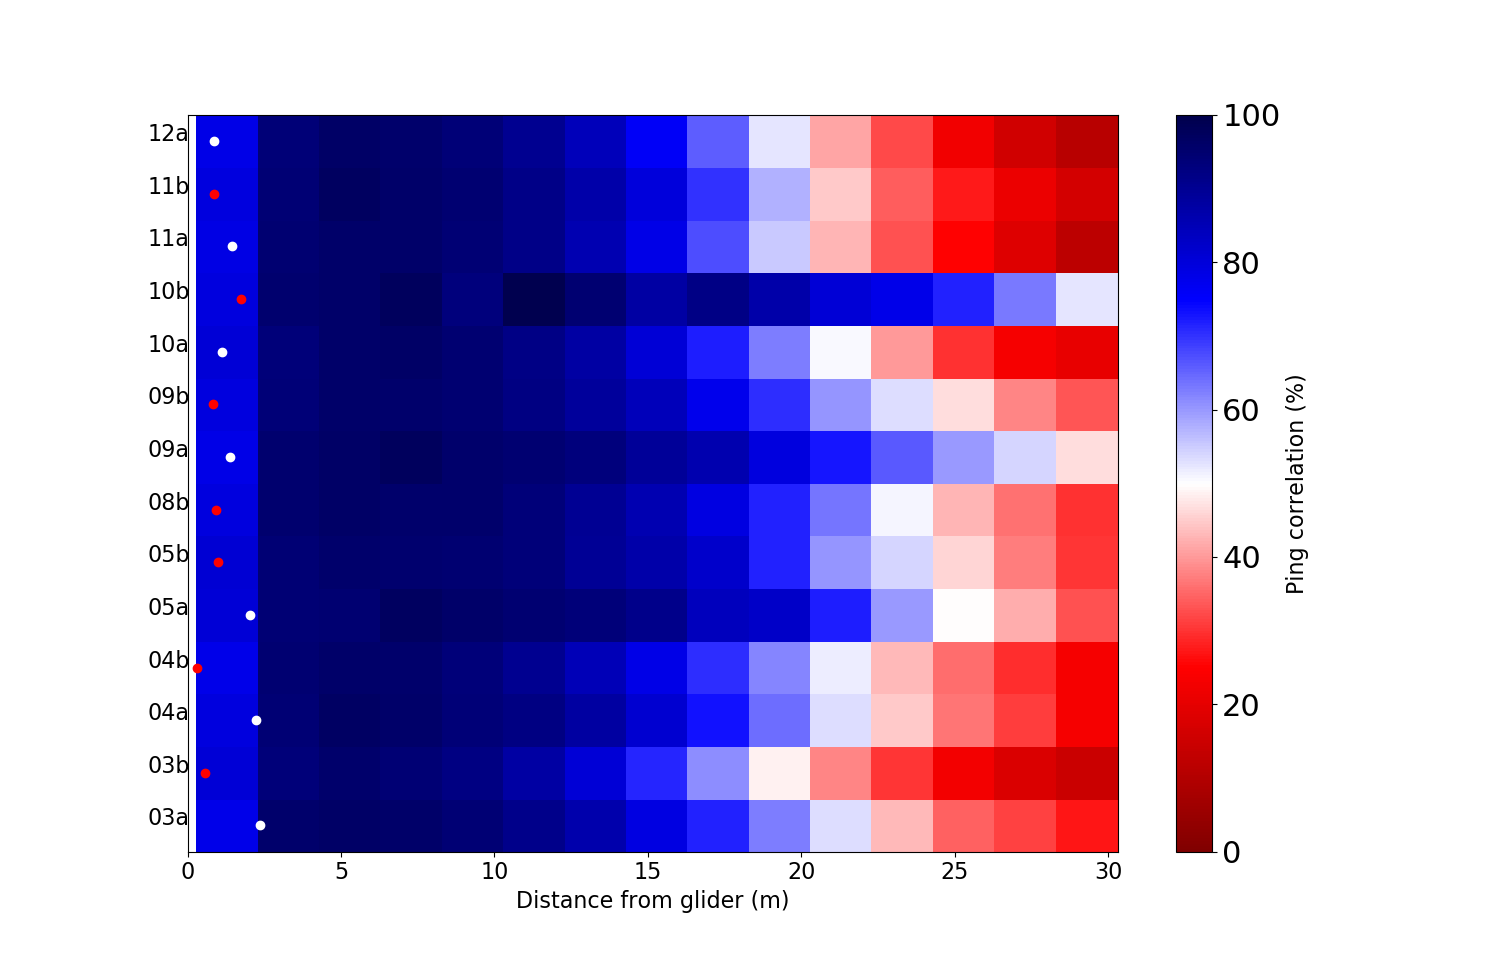
\includegraphics[trim=0 10 0 50,clip,width=0.8\textwidth,keepaspectratio]{%
figure/corr.png}
\end{center}
\vspace{-0.3cm}
\begin{columns}
\begin{column}[t]{0.9\textwidth}
Average ping correlation over the course of 8 dives. Good correlation is achieved out to 15 - 20 m. Dots are average beam miss 15 m from glider, white for descent, red for ascent, as in \hyperlink{flight_envelope}{\beamerbutton{beam miss from flight}}
\end{column}
\end{columns}
\end{frame}

\begin{frame}\label{no_qc}
\vspace{-0.3cm}
\begin{center}
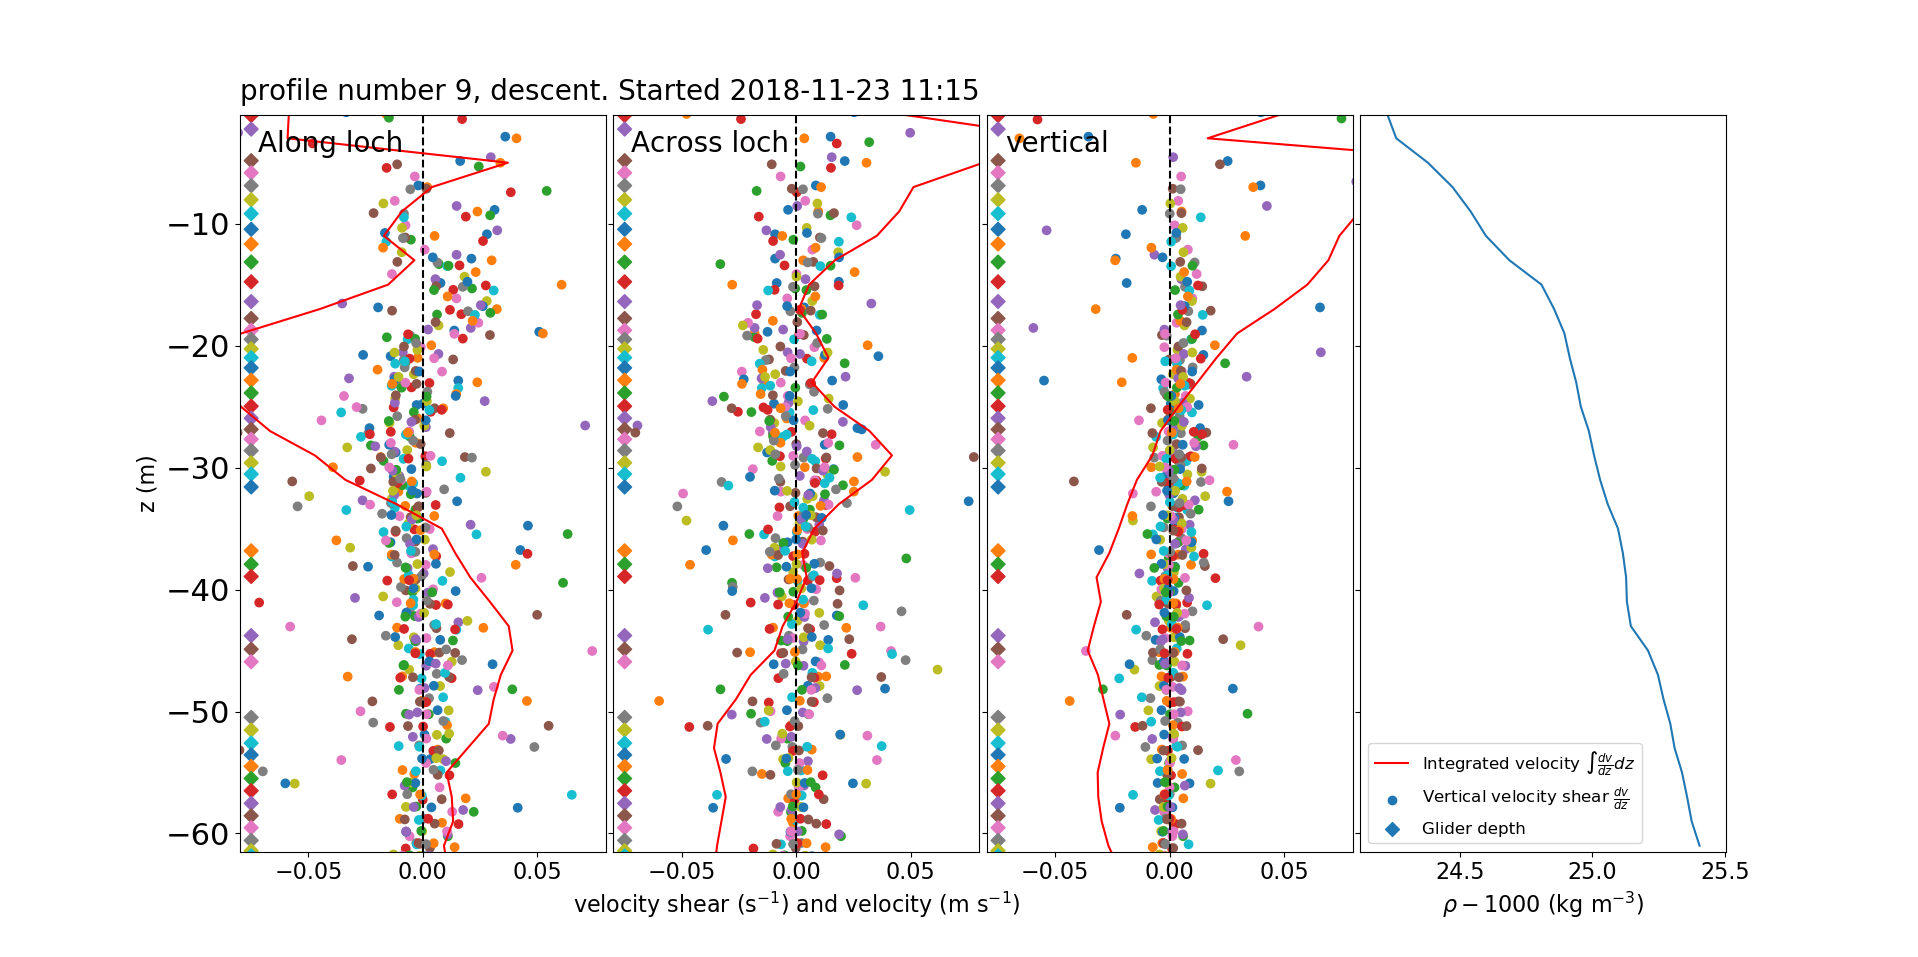
\includegraphics[trim=70 20 80 80,clip,width=\paperwidth]{figure/95_noqc.png}
\end{center}
\begin{columns}
\begin{column}[t]{0.9\textwidth}
The same data as \hyperlink{trial_shear}{\beamerbutton{the introduction}}, without quality control steps. The shape of horizontal shear is visible, but the signal is extremely noisy.
\end{column}
\end{columns}
\end{frame}


%%%%%%%%%%%%%%%%%%%%%%%%%%%%%%%%%%%%%%%%%%%%%%%%%%%%%%%%%%%%%%%%%%%%%%%%%%
\mysection{tech}
%%%%%%%%%%%%%%%%%%%%%%%%%%%%%%%%%%%%%%%%%%%%%%%%%%%%%%%%%%%%%%%%%%%%%%%%%%
\begin{frame}\label{\secvariable}

\begin{columns}
\begin{column}[t]{0.9\textwidth}
\ \textbf{Seaglider spec:} max depth 1000 m , vertical velocity $\approx0.1\ \mathrm{m\ s^{-1}}$

\ \textbf{ADCP spec/deployment settings:}
\begin{itemize}
\item Sampling frequency 1 MHz 
\item Range 30 m (max) 15-20 m (typical)
\item 3 downward facing beams at 30 degrees from vertical 
\item Cell size 2 m
\item Blanking distance 0.3 m
\item 3 second ensemble of 8 pings every 30 seconds
\end{itemize}
Gives 80 - 85 \% profile overlap (15-20 m range velocity shear profile every 3 m of glider vertical travel)

Expected endurance 6 weeks \hyperlink{animation}{\beamerbutton{Take me back to the cool animation}}
\noindent\rule[0.5ex]{\linewidth}{1pt}

\usebeamerfont{bodytext}
\LaTeX{} available on my github  \texttt{github.com/callumrollo/pico-latex-presentation}
Adapted from the template by Anselm K\"ohler: \texttt{github.com/snowtechblog/pico-latex-presentation}
\end{column}
\end{columns}
\end{frame}



\end{document}
